\section{Ressourcenplanung}
\subsection{Meilensteine}
Unser Team hat sich darauf geeinigt, dass der Projektleiter über die gesamte Zeit bei derselben Person bleibt.
So ist immer klar wer den Überblick haben muss und es gibt keine Wissens-Verluste bei der Übergabe des Projektstandes zwischen Projektleitern. 

\begin{tabularx}{\textwidth-2cm}{|l|l|X|} \hline
\textbf{Meilenstein}	& \textbf{Verantwortlichkeit} &	\textbf{Erwartung} \\ \hline
\textbf{M1}	&Sascha Bergmann	&Vorschau GUI, Datenbank (ER-Schema) \\  \hline
\textbf{M2}	&Sascha Bergmann	&Design und DB umgesetzt; mind. Ein Hauptprozess vollständig umgesetzt \\ \hline
\textbf{M3}	&Sascha Bergmann	&Hauptprozesse umgesetzt; Codierungsstil/Modularisierung \\ \hline
\textbf{M4}	&Sascha Bergmann	&Abnahmetests; Gruppenspezifischer Schwerpunkt \\ \hline
\textbf{M5}	&Sascha Bergmann	&Präsentation der Arbeit \\ \hline
\end{tabularx}

\iffalse
  \begin{ganttchart}{1}{12}
    \gantttitle{Projektplan}{12} \\
    \gantttitlelist{1,...,12}{1} \\
    \ganttmilestone{Meilenstein M1}{4}  \ganttnewline
    \ganttmilestone{Meilenstein M2}{5}  \ganttnewline
    \ganttmilestone{Meilenstein M3}{6}  \ganttnewline
    \ganttmilestone{Meilenstein M4}{7} 
  \end{ganttchart}
\fi

\subsection{Auslastung}
Die Auslastung ist bei allen Personen sehr ähnlich. Der Projektleiter Sascha Bergmann hat ein paar Stunden weniger als die anderen Teammitglieder. Dies ist absichtlich so gelöst, da der Projektleiter noch Zeit benötigt administrative Arbeiten auszuführen, wie z.B. Vorbereitung von Meilenstein-Sitzungen, Arbeitsstände überprüfen, eventuelle Planungsänderungen vornehmen.

\definecolor{bergmansas}{HTML}{5B9BD5}
\definecolor{kunzlio}{HTML}{ED7D31}
\definecolor{muellcy1}{HTML}{A5A5A5}
\definecolor{nguyeda}{HTML}{FFC000}

\begin{figure}[H]
\centering
\pgfplotstableread{
MS    bergmansas     kunzlio    muellcy1    nguyeda
1     13.75          13.75      18.75       13.75
2     10             12         11          20
3     12             17         16          10
4     12.5           12.5       12.5        12.5
}\datatable

\begin{tikzpicture}
\begin{axis}[
	width=\linewidth-2cm,
	xbar stacked,
	area legend,
	ytick=data,
	yticklabels={Aufwand M1,
				Aufwand M2,
				Aufwand M3,
				Aufwand M4,
				%\emph{Total}
				},
	legend style={
		legend columns=2,
		at={(xticklabel cs:0.5, 20)},
		anchor=north,
		draw=none
	},
	xlabel={Aufwand in Stunden},
	xticklabel pos=lower,
	minor x tick num=1,
	xmin=0,
	xmax=65,
	bar width=4mm,
	y=7.5mm,
	enlarge x limits={abs=0},
	enlarge y limits={abs=0.7},
	grid=major,
	y dir=reverse,
    point meta=explicit,
    %calculate offset/.code={
    %    \pgfkeys{/pgf/fpu=true,/pgf/fpu/output format=fixed}
    %    \pgfmathsetmacro\testmacro{(\pgfplotspointmeta*10^\pgfplots@data@scale@trafo@EXPONENT@x)/2*\pgfplots@x@veclength)}
    %    \pgfkeys{/pgf/fpu=false}
    %},
    %every node near coord/.style={
    %    /pgfplots/calculate offset,
    %    yshift=-\testmacro
    %},
	%nodes near coords,
	%nodes near coords align=center
]
\addplot[bergmansas,fill=bergmansas] table [y={MS}, x=bergmansas] \datatable;
\addplot[kunzlio,fill=kunzlio] table [y={MS}, x=kunzlio] \datatable;
\addplot[muellcy1,fill=muellcy1] table [y={MS}, x=muellcy1] \datatable;
\addplot[nguyeda,fill=nguyeda] table [y={MS}, x=nguyeda] \datatable;
\legend{S. Bergmann, L. Kunz, C. Müller, D. Nguyen}
\end{axis}
\end{tikzpicture}
\caption{Auslastung pro Meilenstein.}
\end{figure}



\begin{figure}[H]
\centering
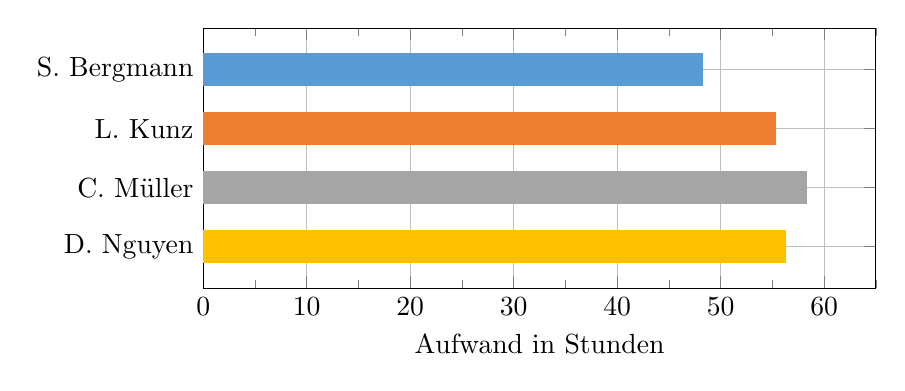
\begin{tikzpicture}
\centering
\begin{axis}[
	width=\linewidth-2cm,
	xbar stacked,
	area legend,
	ytick=data,
	yticklabels={S. Bergmann,
				L. Kunz,
				C. Müller,
				D. Nguyen,
				\emph{Total}
				},
	xlabel={Aufwand in Stunden},
	xticklabel pos=lower,
	minor x tick num=1,
	xmin=0,
	xmax=65,
	bar width=4mm,
	y=7.5mm,
	enlarge x limits={abs=0},
	enlarge y limits={abs=0.7},
	grid=major,
	y dir=reverse
]
\addplot[bergmansas,fill=bergmansas, x={label}, y={bergmansas}] coordinates
% Transfer
{%(13,0)
(48.25, 0)
(0,1)
(0,2)
(0,3)
};

\addplot[kunzlio,fill=kunzlio] coordinates
{
(0,0)
(55.25,1)
(0,2)
(0,3)
};

\addplot[muellcy1,fill=muellcy1] coordinates
{
(0,0)
(0,1)
(58.25,2)
(0,3)
%(18.75,0)
%(11,1)
%(16,2)
%(12.5,3)
%(,4)
};

\addplot[nguyeda, fill=nguyeda] coordinates
{
(0,0)
(0,1)
(0,2)
(56.25,3)
%(,4)
};

%\legend{Sascha Bergmann, Lion Kunz, Cyril Müller, Dang Thien Nguyen}

\end{axis}
\end{tikzpicture}
\caption{Gesamte Auslastung pro Person.}
\end{figure}

\iffalse % auskommentieren der jpg diagramme
\begin{figure}[H]
\centering
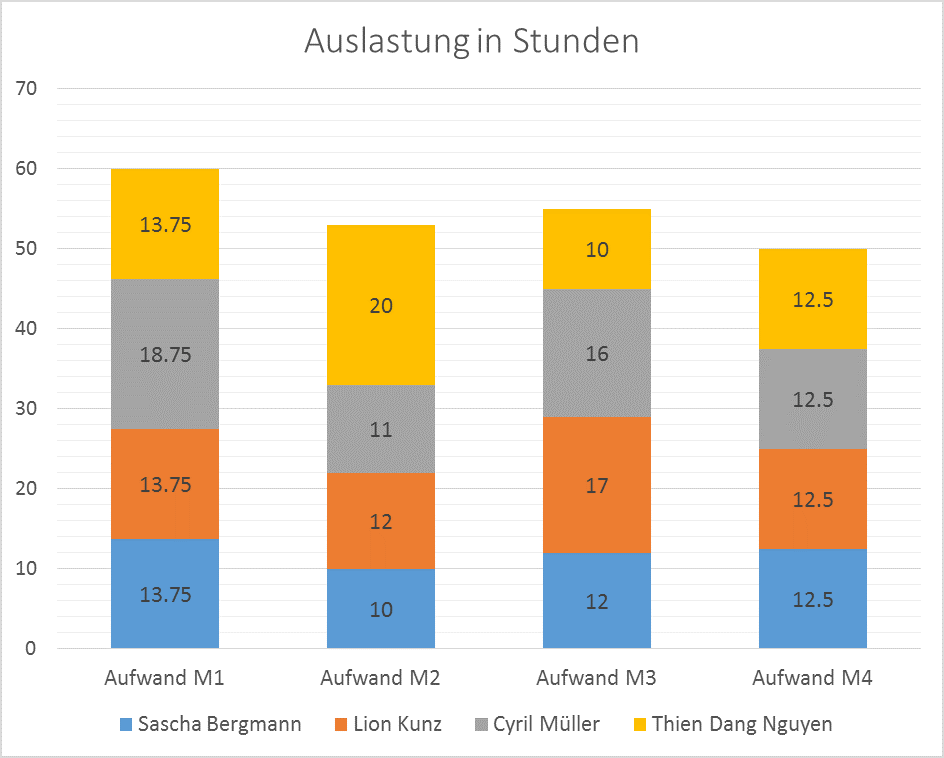
\includegraphics[width=0.7\textwidth]{graphics/auslastung_meilensteine.png}
\caption{Aufwand pro Meilenstein.}
\end{figure}


\begin{figure}[H]
\centering
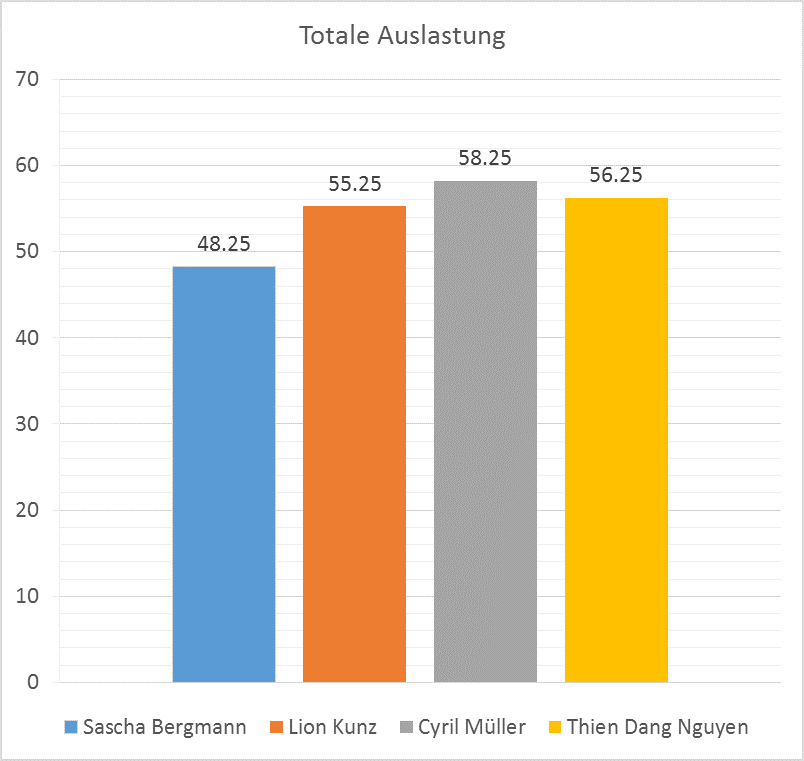
\includegraphics[width=0.7\textwidth]{graphics/auslastung_total.png}
\caption{Aufwand pro Person.}
\end{figure}
\fi